\section{Motivation}
\label{motivation}

In this section, we demonstrate the main problem when running the graph 
coloring algorithms on GPU, which motivate us to develop Feluca. 

According to previous studies, the graph coloring algorithms can be divided into 
several categories, in which \textit{sequential spread} and \textit{recursion} are most often used \cite{sequential,recursion}. 

The basic idea 
%Most existed research on graph coloring are traversal based algorithms, the basic 
of the sequential spread algorithm is to traverse the entire graph using the algorithms such as BFS, and check the 
vertex's color one by one. These algorithms proceed in synchronized steps and use the 
threads to work on the active vertices.  A crucial attribute of a synchronous computing model is the number of synchronized steps. An algorithm that has a less number of synchronized steps delivers the better performance. 

In the sequential spread model, each synchronized step can be divided into three phase. In the first phase, the colored vertices need to send 
their colors to their neighbouring vertices. In the second phase, the neighbours receive the message about the colors and then in the third phase, the neighbours execute the local computation. However, we observed from our benchmarking experiments that although the number of synchronized steps is large,
there are only a small number of active vertices in each step. Moreover, it is difficult to run this execution model in parallel, because the active vertices in current iteration can be colored only when the results of previous iterations are known.


The other type of graph coloring algorithms employs the recursive execution, which works in a similar way as PageRank. %iterative execution 
High performance recursion-based graph coloring algorithms have been developed in recent works \cite{iterative,Manycore}. %, which executed iteratively. 
In this coloring model, every vertex is assigned a color at the beginning. Then every vertex sends its 
color value to its neighbours. Next, the neighbouring vertex updates its color if the color conflicting occurs (i.e., the neighbouring vertices have the same color). 

The colors of most vertices converge in the first few iterations. The remaining small fraction of vertices take a long time to converge to the final color due to color conflicts. This \textit{long-tail} 
phenomenon can be demonstrated from the following benchmark experiments. We ran the experiments on a NVIDIA Tesla K20m GPU, which is equipped with 5 GB on-board memory, 2,496 CUDA 
cores, and Red Hat Enterprise Linux Server release 6.2 (Linux version 3.10.0-514.el7.x86\_64). 
As shown in figure \ref{fig:colored_vertices_Iter}, the number of vertices that are colored in each iteration drops dramatically in the first few iterations (i.e., these vertices converge to their final colors) and only a very small fraction of vertices are active in a large number of remaining iterations. Take the youtube dataset as an example. There are 1,157,828 vertices in total. 1,148,571 vertices converge in the first 2 iterations, while the remaining 9,257 vertices take more than 30 iterations to converge. We also plot the ratio of the number of conflicting vertices to the number of active vertices in each iteration, shown in figure \ref{fig:conflict_vertices}. The ratio is only 4\% in the first iteration, and increases to 92.3\% in the $26^{th}$ iteration. These results suggest the recursion algorithm is very effective in the first few iterations, but does not conduct much useful work in the remaining iterations. This work aims to address this problem. 

\begin{figure}
\centering
%\subfloat[Iteration algorithm]{%
\subfloat[Colored vertices]{%
\label{fig:colored_vertices_Iter}
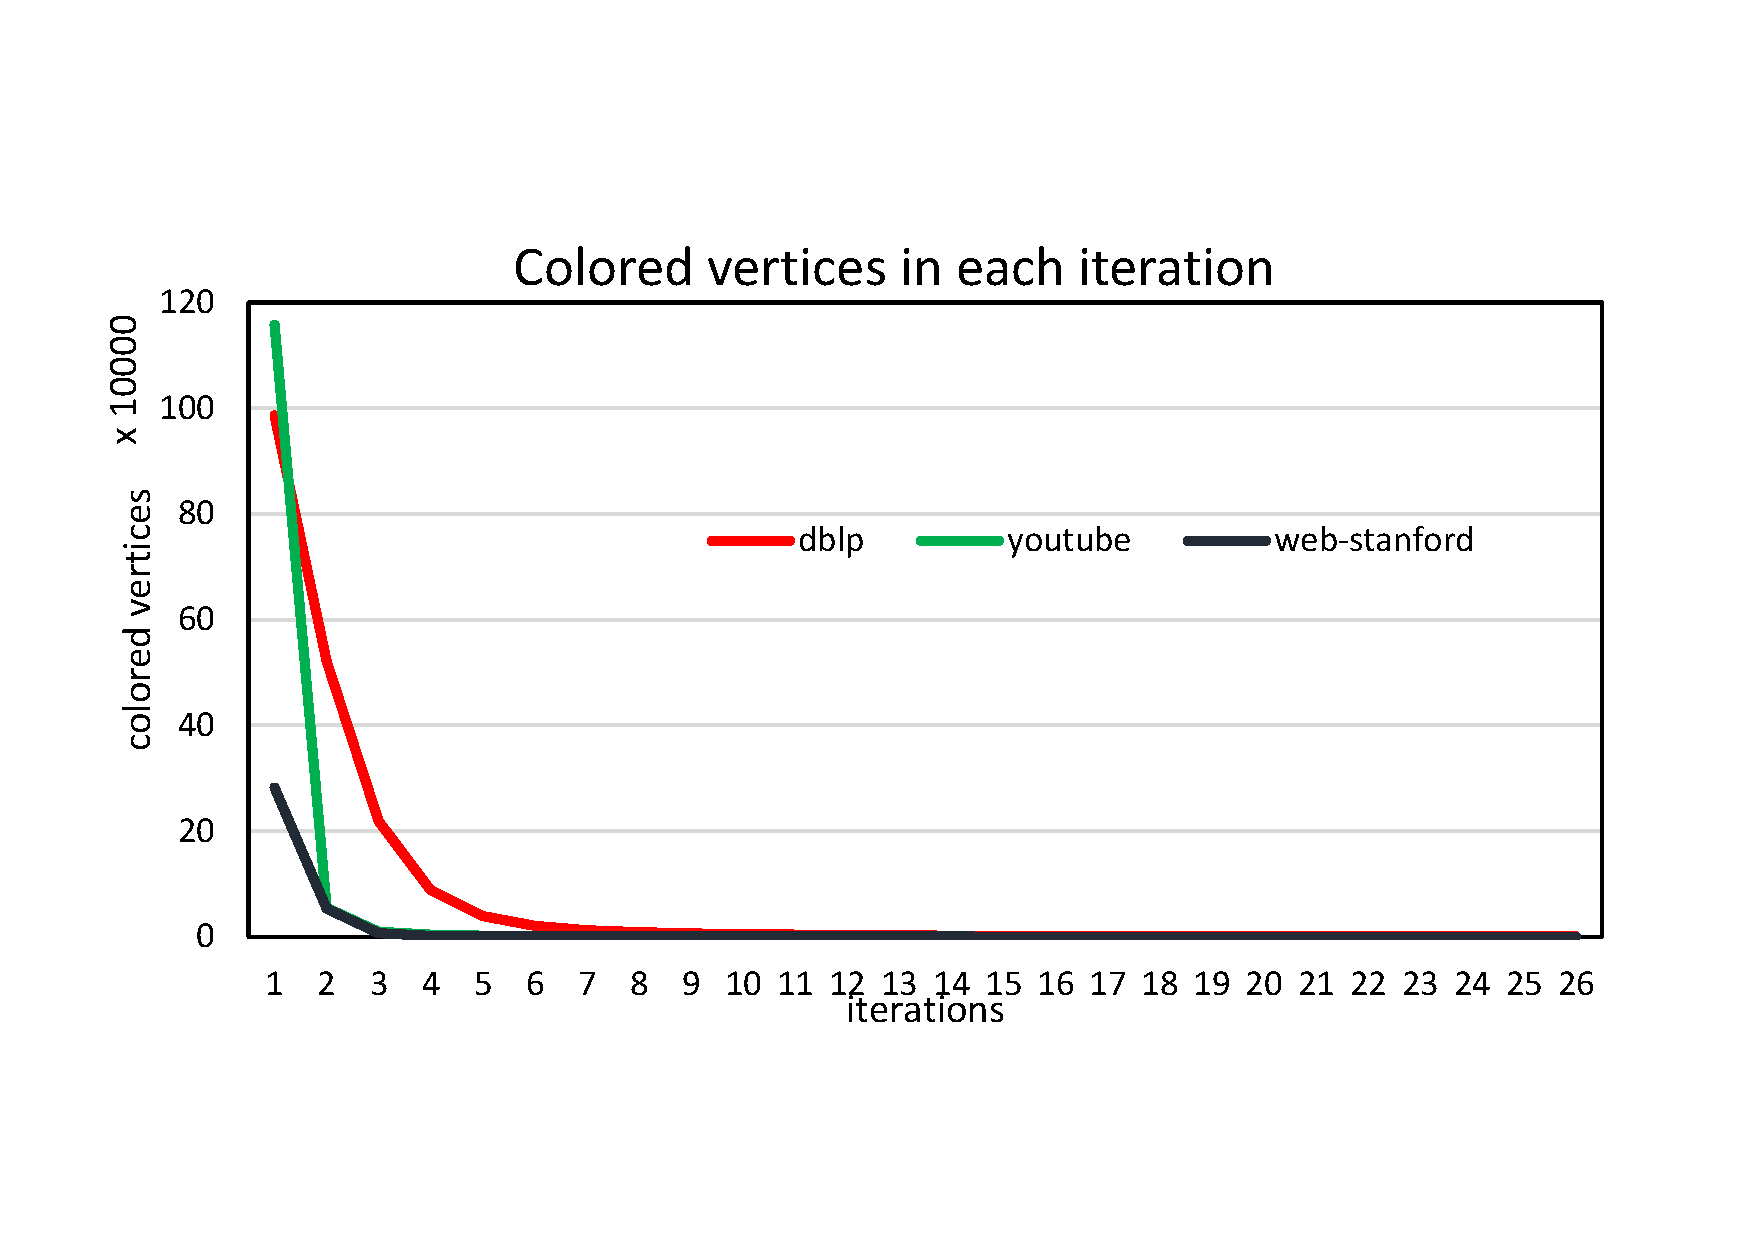
\includegraphics[scale=0.15]{figure/colored_vertices.pdf}
}%
\subfloat[Vertices conflict rate]{
\label{fig:conflict_vertices}
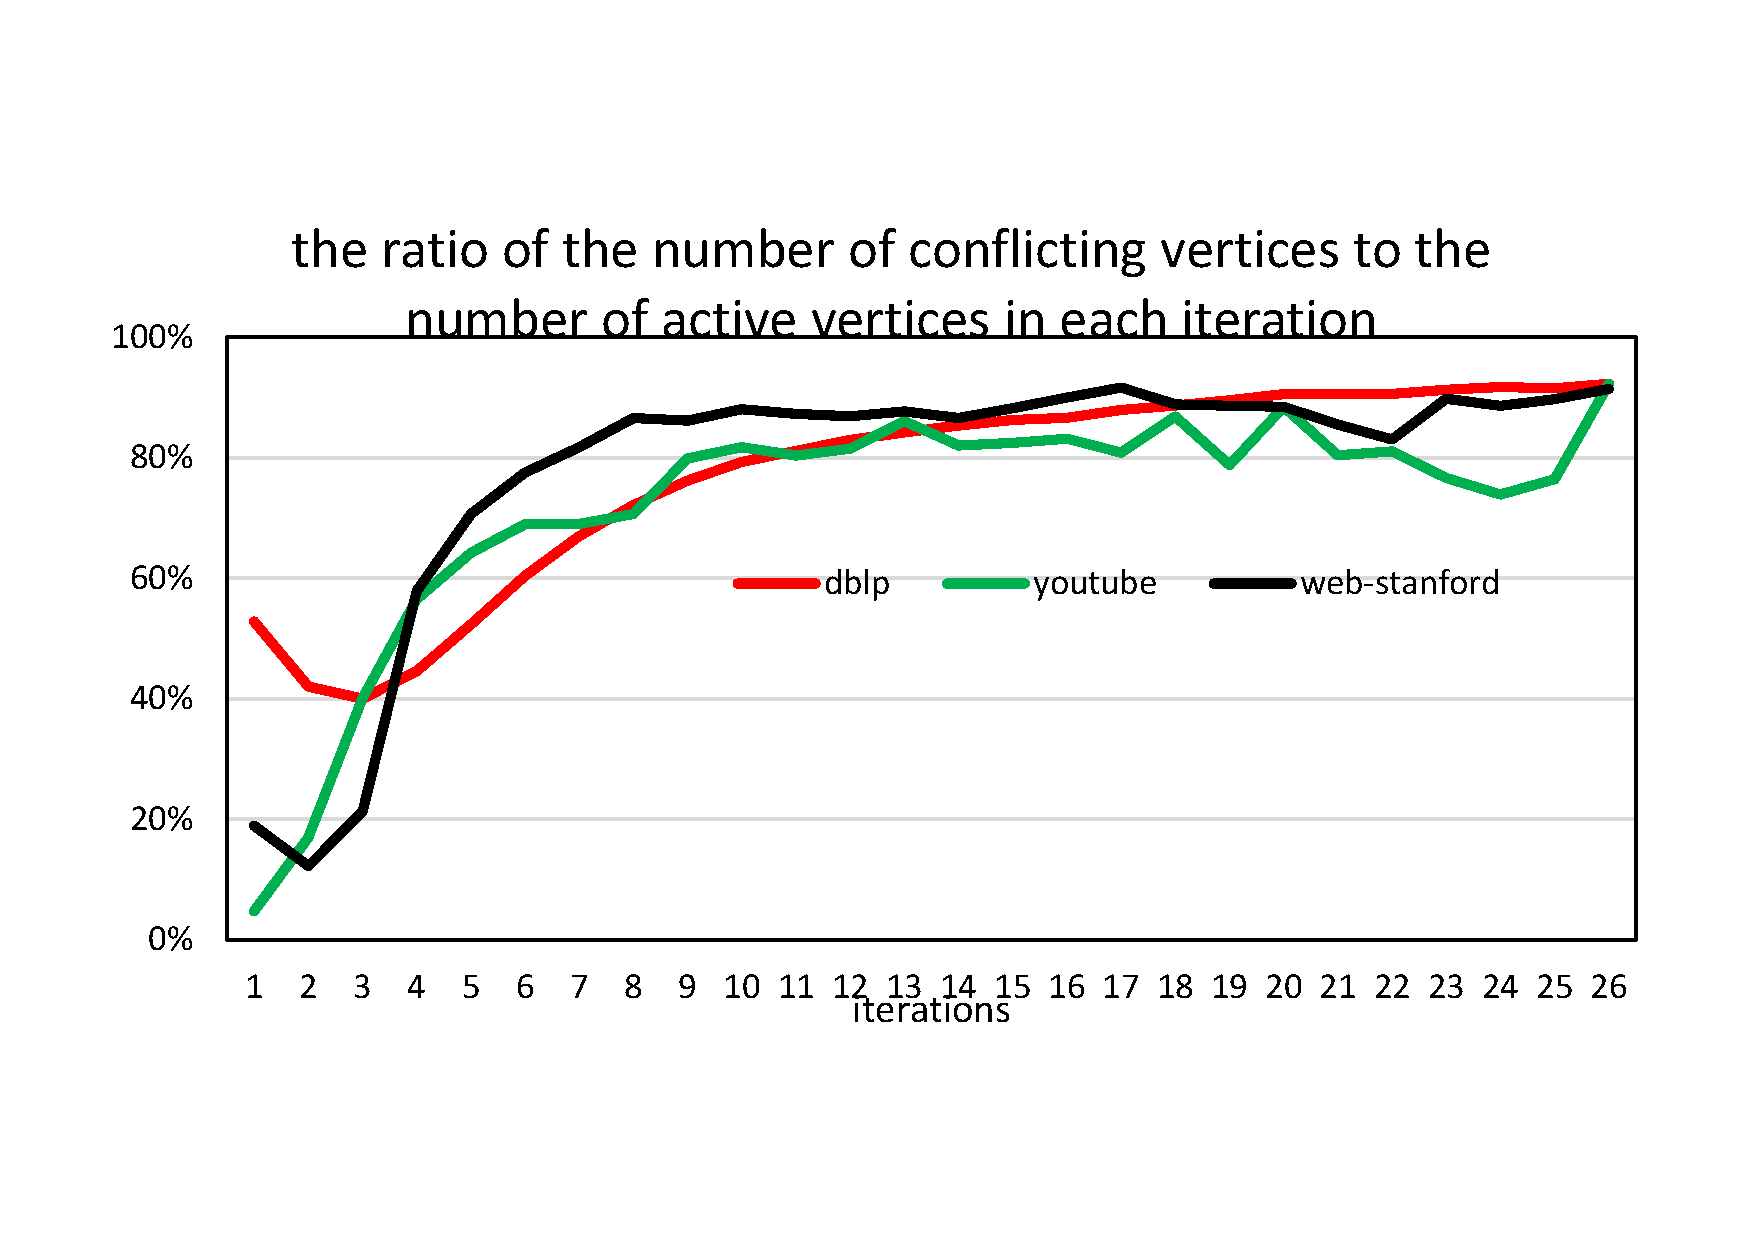
\includegraphics[scale=0.15]{figure/conflict_vertices.pdf}
}%
\caption{The number of colored vertices (Figure \ref{fig:colored_vertices_Iter}) and the ratio of the number of conflicting vertices to the number of active vertices ( figure \ref{fig:conflict_vertices}) as the graph coloring process progress through each iteration. }
\label{fig:colored_vertices}%
\end{figure}

%讲遍历型算法的问题

%In order to demonstrate the problem of sequential spread graph coloring problem, we have conducted the following benchmark experiments. The experiment platform includes a NVIDIA Tesla K20m GPU which equipped with 5 GB on broad memory and 2,496 CUDA cores, and running on Red Hat Enterprise Linux Server release 6.2 (Linux version 3.10.0-514.el7.x86\_64). As we shown in figure \ref{fig:colored_vertices_Tra} the number of colored vertices in each synchronized step is relatively low. From the figure we can conclude that the peak and trough value of the colored vertives are stay in a narrow space except the first few synchronized steps. Which indicates that the active vertices stays almost the same in most synchronized steps.

%讲迭代型算法的问题

Moreover, most recent studies in literature  \cite{Manycore} apply \textit{atomic} operations to implement parallel coloring algorithms on both CPU and GPU. This implementation method greatly restricts the degree of parallelism on GPU. Therefore, it is very useful to develop a graph coloring algorithm that can fully unleash the power of GPU. 
